% ! TeX root = ../bachelor-thesis.tex

\chapter{Progettazione del sistema}
\label{ch:Chapter3}

In questo capitolo si proporrà una possibile soluzione che soddisfa i requisiti
\textit{must have} del sistema descritto precedentemente.

Più in dettaglio, si analizzeranno le tecnologie scelte per implementare il
sistema, focalizzandosi prima sul loro funzionamento individuale e
successivamente su come possono interagire tra di loro. Inoltre, sarà
giustificata la scelta di tali tecnologie nel contesto in cui è stato
sviluppato il progetto. Infine, si illustreranno alcune possibili limitazioni
del sistema, non più dipendenti dalla natura del problema stesso, ma derivanti
dalle tecnologie specifiche utilizzate per implementarlo.

\section{Architettura del Sistema}
\label{sec:Sezione3.1}

Ora si descriverà una possibile soluzione al problema introdotto nei capitoli
precedenti, facendo riferimento ai requisiti \textit{must have} del sistema.

In particolare, si progetterà prima un’architettura di massima che descriva
quali sono i componenti e le interazioni che appartengono al sistema, dopodiché
s’illustrerà l’architettura effettivamente implementata, vincolata alle
specifiche tecnologie scelte.

\subsection{Architettura di massima}
\label{subsec:Sezione3.1.1}

Di seguito, viene proposta un’architettura generica di massima che possa
soddisfare i requisiti \textit{must have} del problema (Figura
\ref{fig:figure3.1}).

\begin{figure}[!ht]
  \centering
  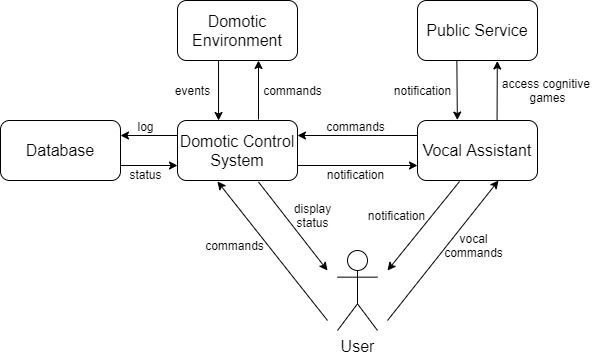
\includegraphics[scale=0.7]{resources/images/design/system-structure-analysis-diagram.jpg}
  \caption{Lo schema delle interazioni in una generalizzazione del sistema.}
  \label{fig:figure3.1}
\end{figure}

L’\textbf{utente} potrà interfacciarsi con il sistema attraverso il
\textbf{sistema di controllo domotico} e l’\textbf{assistente vocale}. Entrambi
gli permetteranno di controllare il proprio \textbf{ambiente domotico},
composto da tutti i dispositivi domotici del sistema. Il sistema di controllo
domotico registrerà anche gli eventi ricevuti dall’ambiente domotico in un
\textbf{database} e consentirà all’utente di accedere allo stato corrente e
allo storico degli stati dei suoi dispositivi domotici. Inoltre, potrà
notificare l’utente di certi eventi accaduti, attraverso messaggi vocali
mediati dall’assistente vocale. L’assistente vocale, oltre a delegare i comandi
vocali rivolti verso l’ambiente domotico al sistema di controllo domotico,
permetterà l’accesso agli esercizi cognitivi. Questi saranno esposti attraverso
un \textbf{servizio pubblico}, quindi accessibile dall’assistente vocale.

\subsection{Progetto del sistema}
\label{subsec:Sezione3.1.2}

Dopo aver descritto l’architettura di massima, ora si riporterà un’architettura
vincolata alle tecnologie scelte per implementare il sistema (Figura
\ref{fig:figure3.2}).

\begin{figure}[!ht]
  \centering
  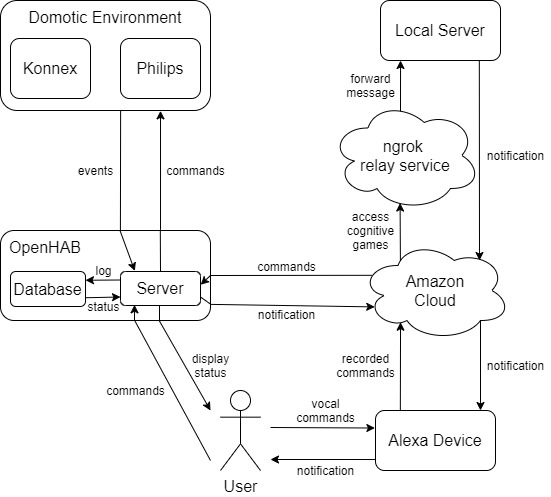
\includegraphics[scale=0.6]{resources/images/design/system-structure-design-diagram.jpg}
  \caption{
    Lo schema delle interazioni nel sistema che sarà implementato in questo
    elaborato.
  }
  \label{fig:figure3.2}
\end{figure}

Più in dettaglio, le tecnologie scelte sono:
\begin{itemize}
  \item[--] Per l’\textit{ambiente domotico}, si è scelta una smart home
        composta da un impianto domotico \textbf{KNX} \cite{KONNEX} e alcuni
        dispositivi smart della \textbf{Philips} \cite{PHILIPS}. Questo
        sistema era già predisposto su di un appartamento usato come caso di
        studio;
  \item[--] Per il \textit{sistema di controllo domotico}, è stato scelto
        \textbf{OpenHAB} \cite{OPENHAB}, perché consente di gestire una grande
        varietà di dispositivi domotici e quindi di non vincolarsi a uno
        specifico produttore. In aggiunta, è anche comprensivo di un database.
        Questo sistema era in gran parte già predisposto per controllare
        l’appartamento domotico;
  \item[--] Per l’\textit{assistente vocale}, è stata scelta \textbf{Amazon
          Alexa} \cite{ALEXA}, nello specifico un dispositivo
        \textit{\textbf{Alexa Echo Dot}}, poiché già disponibile da ricerche
        e studi precedenti;
  \item[--] Per gli \textit{esercizi cognitivi}, allo scopo di eliminare i
        costi di manutenzione di un server pubblico, è stato scelto
        d'implementare un servizio su un server locale, esposto come server
        pubblico tramite \textbf{ngrok} \cite{NGROK}, ovvero un servizio
        gratuito in cloud che inoltra le richieste ricevute a una specifica
        porta di una macchina locale.
\end{itemize}

\section{Tecnologie utilizzate}
\label{sec:Sezione3.2}

In questo capitolo, si entrerà più nel dettaglio rispetto alle tecnologie
utilizzate nel progetto, spiegando come vengono realizzate le interazioni tra i
vari componenti del sistema.

Dunque, saranno prima descritte le caratteristiche di OpenHAB, come sistema di
controllo domotico, poi di Alexa, come assistente vocale, e infine saranno
descritti i servizi che offrono per interfacciarsi l’uno con l’altro.

\subsection{OpenHAB come sistema di controllo domotico}
\label{subsec:Sezione3.2.1}

\textbf{OpenHAB} (Open Home Automation Bus) è una piattaforma che gestisce la
comunicazione e l’automazione in un ambiente domotico, svincolandosi dalle
specifiche tecnologie utilizzate dai dispositivi che controlla. Le sue
caratteristiche principali sono:
\begin{itemize}
  \item[--] La possibilità d'\textit{integrare dispositivi domotici anche
          molto diversi}, permettendo loro di comunicare indirettamente,
        persino se usano tecnologie e/o protocolli direttamente
        incompatibili;
  \item[--] La possibilità di controllare il proprio ambiente domotico
        attraverso un’\textit{unica interfaccia utente} e di creare
        \textit{regole di automazione per la casa uniche e valide su tutto il
          sistema}, evitando di utilizzare un’applicazione diversa per ogni
        specifico produttore;
  \item[--] È un software \textit{open source}, quindi, oltre a essere
        gratuito, possiede una comunità di sviluppatori che estendono
        continuamente le sue funzionalità. \cite{OPENHAB_DOC}
\end{itemize}

\subsubsection{3.2.1.1. La comunicazione con i dispositivi domotici}
\label{subsec:Sezione3.2.1.1}

La struttura con cui OpenHAB consente l’interazione con i dispositivi connessi,
si basa su diversi livelli d'interfacciamento (come descritto in Figura
\ref{fig:figure3.3}).

\begin{figure}[!ht]
  \centering
  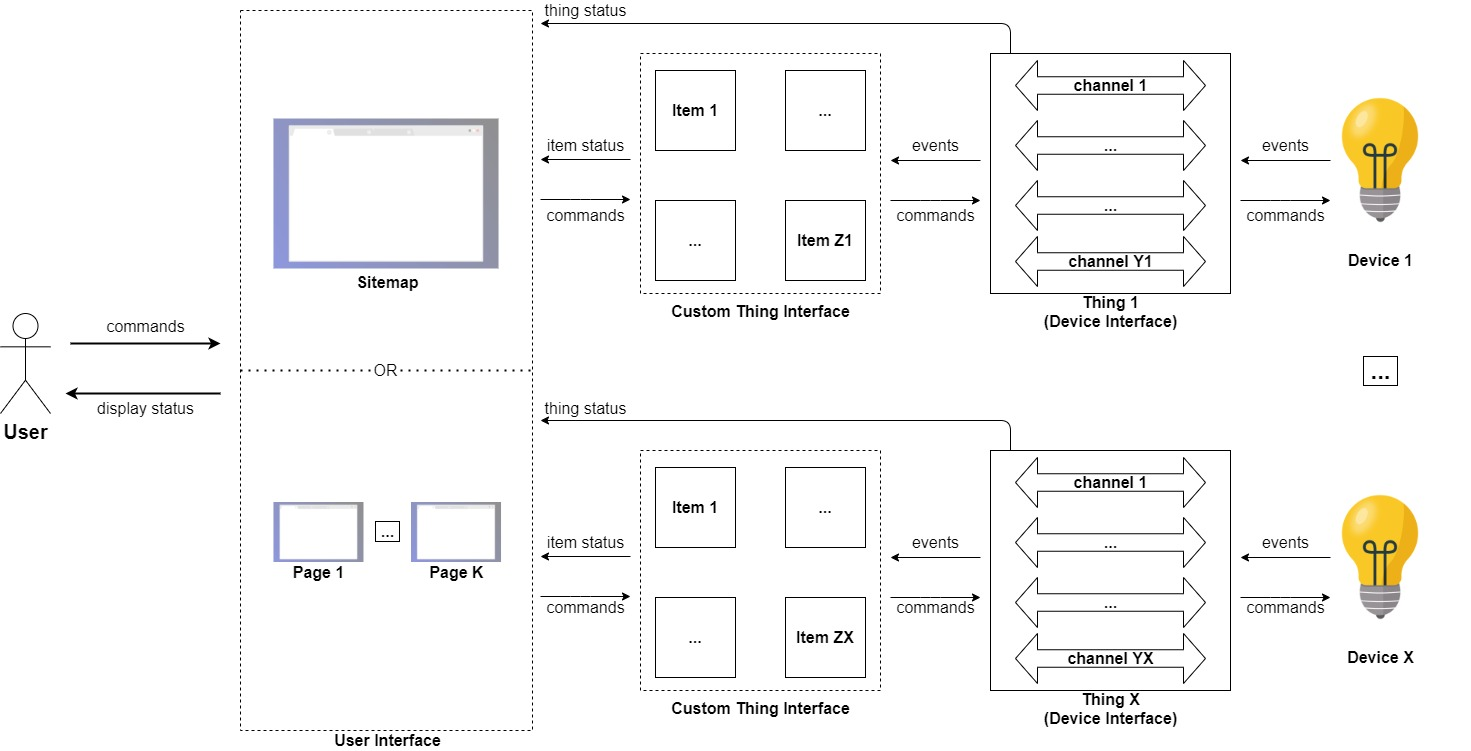
\includegraphics[scale=0.3]{resources/images/other/openhab-control-flow.jpg}
  \caption{
    I diversi livelli d'interfacce poste tra l'utente e i suoi dispositivi
    domotici in OpenHAB.
  }
  \label{fig:figure3.3}
\end{figure}

Il primo livello d'interfacciamento è costituito dalle \textit{\textbf{things}}
\cite{THINGS}, che espongono le funzionalità di un dispositivo fisico
all’interno di OpenHAB, attraverso i \textit{\textbf{channel}} di cui sono
composte. Ciascun \textit{channel} espone una specifica funzione del
dispositivo domotico. Ogni \textit{thing} mantiene lo stato della connessione
tra il dispositivo fisico che controlla e OpenHAB, ad esempio se il dispositivo
è raggiungibile (\textit{ONLINE}) o meno (\textit{OFFLINE}).

Il secondo livello d'interfacciamento è costituito dagli
\textit{\textbf{items}} \cite{ITEMS}. Esistono diversi tipi di \textit{item},
ognuno dei quali si distingue per gli stati che può assumere e i comandi che
può ricevere. Un \textit{item} può essere associato a più \textit{channel}, che
controllerà inoltrando loro i comandi che riceve. Viceversa, un
\textit{channel} può essere associato a più \textit{item}, da cui sarà
controllato. Gli \textit{item} offrono un certo grado di libertà e permettono
di scegliere con quali comandi si vuole controllare i propri dispositivi, al
contrario delle \textit{thing}, che sono spesso vincolate dal dispositivo
fisico che rappresentano.

L’ultimo livello d'interfacciamento è costituito dall'\textbf{interfaccia
utente}, esposta attraverso il \textit{Web Server di OpenHAB} e quindi
accessibile tramite browser. All’interno di OpenHAB ne esistono di diversi
tipi, ma le più recenti sono:
\begin{itemize}
  \item \textit{\textbf{Sitemap}} \cite{SITEMAP}: un’interfaccia dalla grafica
        minimale e funzionale;
  \item \textit{\textbf{Pages}} \cite{PAGES}: un’interfaccia dalla grafica più
        accattivante e user-friendly.
\end{itemize}
Le componenti grafiche con cui si controlla un \textit{item} dall’interfaccia
utente sono determinate dal tipo di quell’\textit{item}.

Di seguito, si riporta un esempio che integra quanto detto finora (Figura
\ref{fig:figure3.4}).
\begin{figure}[!ht]
  \centering
  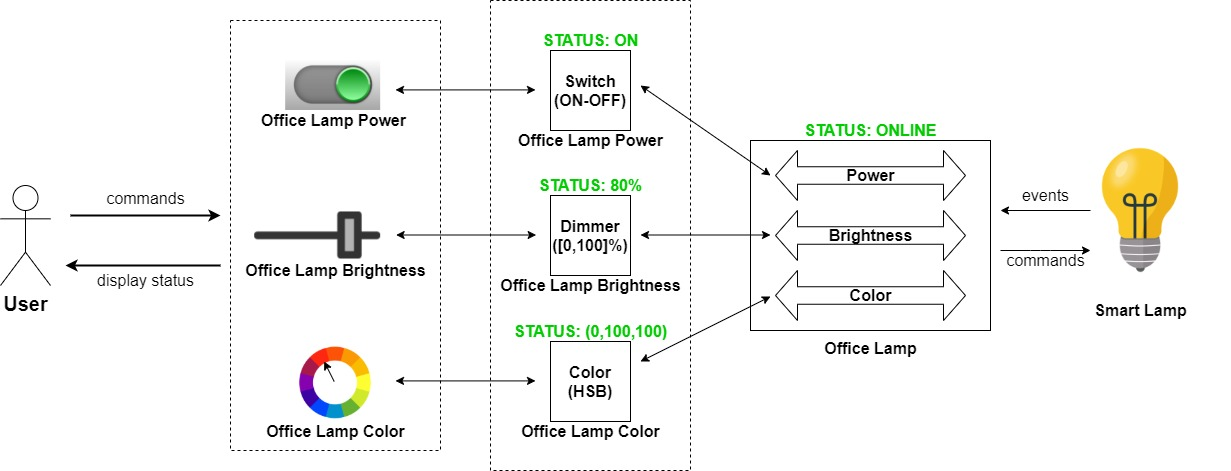
\includegraphics[scale=0.36]{resources/images/other/openhab-lamp-example.jpg}
  \caption{
    Esempio d'interfacciamento tra l'utente e una lampadina smart tramite
    OpenHAB.
  }
  \label{fig:figure3.4}
\end{figure}

\subsubsection{3.2.1.2. Add-On, Automazione e Persistenza}
\label{subsec:Sezione3.2.1.2}

Alle componenti principali, che permettono la comunicazione tra OpenHAB e i
dispositivi domotici, si aggiungono delle componenti più avanzate.

In primo luogo, i \textit{\textbf{binding}} \cite{BINDING} sono degli
\textit{add-on} che aggiungono ulteriori funzionalità a OpenHAB. Normalmente, i
\textit{binding} forniscono nuove tipologie di \textit{thing}, che possiedono
\textit{channel} preconfigurati per connettere a OpenHAB dispositivi di una
certa categoria. Ad esempio, esistono \textit{binding} per dispositivi domotici
di diversi produttori (come \textit{Philips Hue Binding}).

In secondo luogo, le \textit{\textbf{rule}} \cite{RULES} gestiscono la parte di
automazione di OpenHAB. In particolare, sono degli \textit{handler} che possono
accedere e inviare comandi agli \textit{item} in risposta a particolari eventi.

Infine, la \textit{\textbf{persistence}} \cite{PERSISTENCE} consente di
costruire uno storico degli stati e degli eventi ricevuti, memorizzandoli sul
database integrato di OpenHAB. È infatti possibile configurare OpenHAB in modo
che campioni automaticamente lo stato di alcuni \textit{item} indicati. Il
metodo di campionamento può essere descritto attraverso una
\textit{\textbf{strategy}}, che indica ogni quanto e sotto quali condizioni
campionare gli \textit{item}.

\subsection{Alexa come assistente vocale}
\label{subsec:Sezione3.2.2}

\textbf{Amazon Alexa} \cite{ALEXA}, o semplicemente Alexa, è un’assistente
vocale sviluppato da Amazon. Più precisamente, è un servizio del cloud di
Amazon capace d'interpretare la voce umana producendo del testo, e viceversa,
dunque permettendo un’interazione vocale con altri servizi, sotto la sua
mediazione.

Le applicazioni di Alexa sono numerose, ma principalmente includono:
\begin{itemize}
  \item[--] Lo \textit{sviluppo di Alexa Skills}, ovvero di servizi pubblici
        accessibili tramite comandi vocali;
  \item[--] Lo \textit{sviluppo di dispositivi Alexa-Integrated}, ovvero di
        strumenti controllabili attraverso comandi vocali;
  \item[--] L’agevolazione del monitoraggio e della gestione degli ambienti di
        lavoro tramite \textit{Alexa for Business}.
\end{itemize}
In questo progetto, Alexa sarà utilizzata per interagire, oltre che con il
sistema domotico, anche con gli esercizi cognitivi, che saranno quindi
implementati come \textit{\textbf{skills}} di Alexa.

\subsubsection{3.2.2.1. Alexa Skill}
\label{subsec:Sezione3.2.2.1}

Una \textit{skill} di Alexa è composta principalmente da:
\begin{itemize}
  \item[--] Un \textbf{nome d’invocazione}, che la identifica ed è utilizzato
        per accedere alla \textit{skill};
  \item[--] Un \textbf{modello di dialogo}, situato all’interno del cloud di
        Alexa, che indica le intenzioni che l’utente può esprimere
        all’assistente vocale all’interno della \textit{skill};
  \item[--] Un \textbf{modello logico}, situato nell’endpoint specificato, che
        indica quali saranno le reazioni della \textit{skill} in relazione alle
        intenzioni espresse dall’utente;
  \item[--] Un \textit{\textbf{endpoint}}, ovvero un indirizzo URL verso il
        servizio che implementa il modello logico della \textit{skill}.
\end{itemize}

Per interagire con una certa \textit{skill} è necessario richiamare il suo nome
d'invocazione all’interno dei comandi vocali espressi. In alternativa, è
possibile aprirla come un’applicazione qualsiasi (ad esempio, dicendo
\textit{"Alexa, apri Corriere della Sera."}). In tal caso, Alexa si aspetterà
solo comandi compresi nel modello di dialogo di quella \textit{skill}.

L’interazione con una \textit{skill} di Alexa avviene come mostrato in Figura
\ref{fig:figure3.5}.

\begin{figure}[!ht]
  \centering
  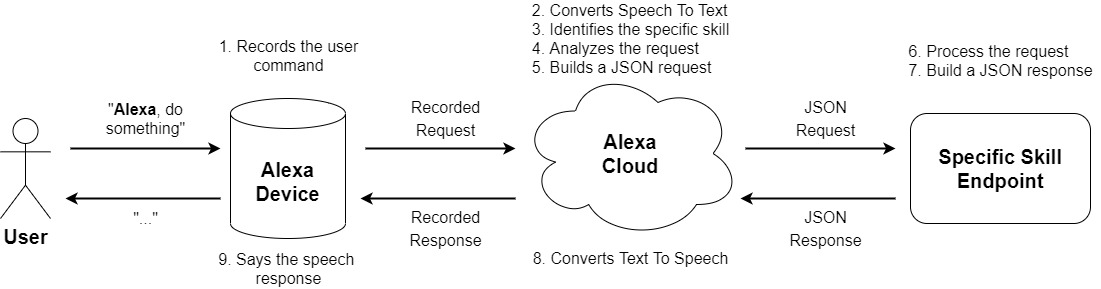
\includegraphics[scale=0.35]{resources/images/other/alexa-skill-flow.jpg}
  \caption{
    Il flusso d'interazione tra l'utente e una \textit{skill} di Alexa che
    permette d'innescare la reazione di un sistema tramite comandi vocali.
  }
  \label{fig:figure3.5}
\end{figure}

Inizialmente, l’utente esprime la propria intenzione a un \textbf{dispositivo
Alexa}, ad esempio un \textit{Alexa Echo Dot}. Per farlo, dovrà precedere il
comando vocale da una \textit{\textbf{wake-word}} (di default
\textit{“Alexa”}), ovvero una parola che indicherà al dispositivo di cominciare
a registrare. Una volta terminata la registrazione del comando vocale, il
dispositivo la inoltrerà al \textbf{cloud di Alexa}, per essere interpretata.
Giunta al cloud di Alexa, la registrazione sarà convertita in un comando
testuale, che sarà analizzato per identificare la \textit{skill} a cui si
riferisce e l’intenzione espressa dall’utente all’interno di quella
\textit{skill}. Il cloud inoltrerà quindi i risultati dell’analisi
all’\textit{\textbf{endpoint}} della \textit{skill} specifica. Ricevuta
l’intenzione dell’utente, l’\textit{endpoint} potrà reagire di conseguenza e
produrre una risposta testuale, che sarà successivamente tradotta dal cloud di
Alexa in una risposta vocale e infine comunicata dal dispositivo Alexa.

Come \textit{endpoint} dove collocare la logica della \textit{skill}, è
possibile scegliere tra diverse soluzioni, come mostrato in Figura
\ref{fig:figure3.6}, ognuna con i propri vantaggi e svantaggi:
\begin{itemize}
  \item[--] \textit{\textbf{Amazon Web Services (AWS) Lambda}}
        \cite{AWS_LAMBDA}: è un servizio in cloud di Amazon che permette di
        eseguire il proprio codice senza dover configurare e mantenere un
        proprio server; è scalabile e facile da usare, tuttavia ha un costo
        mensile basato sul numero di richieste ricevute e sulle risorse
        utilizzate;
  \item[--] Un \textit{\textbf{proprio cloud}}, ovvero un gruppo di cluster di
        macchine gestito in proprio; è scalabile e completamente
        personalizzabile, tuttavia ha una configurazione relativamente più
        lunga e un costo di gestione elevato;
  \item[--] Un \textit{\textbf{proprio server pubblico}}, ovvero una macchina
        accessibile da Internet; è la soluzione meno costosa ed è completamente
        personalizzabile, tuttavia ha una configurazione relativamente più
        lunga e soprattutto non è scalabile, che per un servizio accessibile
        pubblicamente è un grande svantaggio.
\end{itemize}

\begin{figure}[!ht]
  \centering
  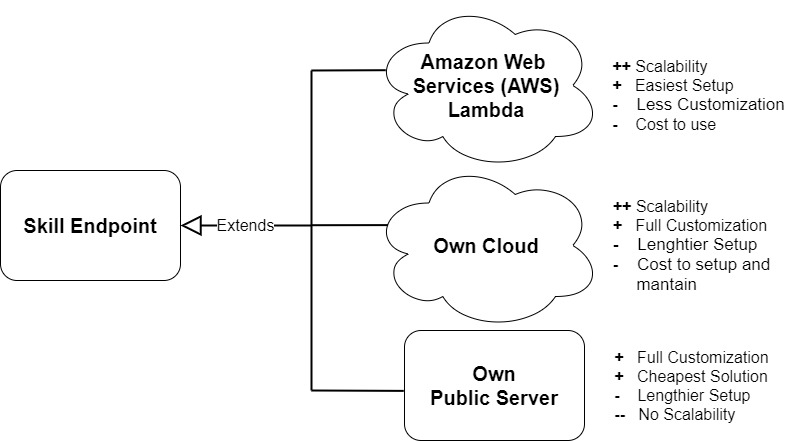
\includegraphics[scale=0.42]{resources/images/other/skill-endpoint-solutions.jpg}
  \caption{
    Le possibili soluzioni adottabili per implementare una \textit{skill} di
    Alexa.
  }
  \label{fig:figure3.6}
\end{figure}

Per minimizzare i costi di progettazione, si è scelta una soluzione a costo
zero, basata su un server locale esposto come server pubblico attraverso il
servizio gratuito \textit{ngrok}.

È possibile sviluppare una nuova \textit{skill} per Alexa interamente
attraverso l’\textbf{Amazon Developer Console} \cite{AMAZON_DEVELOPER_CONSOLE}:
una piattaforma online, gestita da Amazon, che permette l’accesso a diversi
strumenti di sviluppo software. In particolare, per lo sviluppo di una
\textit{skill} esiste uno strumento chiamato \textbf{ASK} (Alexa Skills Kit)
\cite{ASK}.

\subsubsection{3.2.2.2. Il modello di dialogo di una Alexa Skill}
\label{subsec:Sezione3.2.2.2}

Il modello di dialogo di una \textit{skill} di Alexa definisce le intenzioni
(\textit{\textbf{intents}}) che l’utente può esprimere all’interno della
\textit{skill}. Ogni \textit{intent} è associato a una serie di proposizioni
(\textit{\textbf{utterances}}), che l’utente può pronunciare per esprimere
quell’intenzione.

Un \textit{utterance} può contenere degli \textit{\textbf{slot}}, ovvero degli
spazi all’interno della proposizione, identificati da un nome, che possono
assumere un certo dominio di valori, definito dal \textbf{tipo di slot}.

Esistono due categorie a cui può appartenere un tipo di slot:
\begin{itemize}
  \item[--] \textit{Custom slot type}: è un tipo di slot il cui dominio di
        valori è un insieme finito definito dallo sviluppatore della
        \textit{skill};
  \item[--] \textit{Pre-built slot type}: è un tipo di slot il cui dominio di
        valori è predisposto da Amazon.
\end{itemize}

Di seguito, viene riportato uno schema che riassume i componenti appena
descritti (Figura \ref{fig:figure3.7}).
\begin{figure}[!ht]
  \centering
  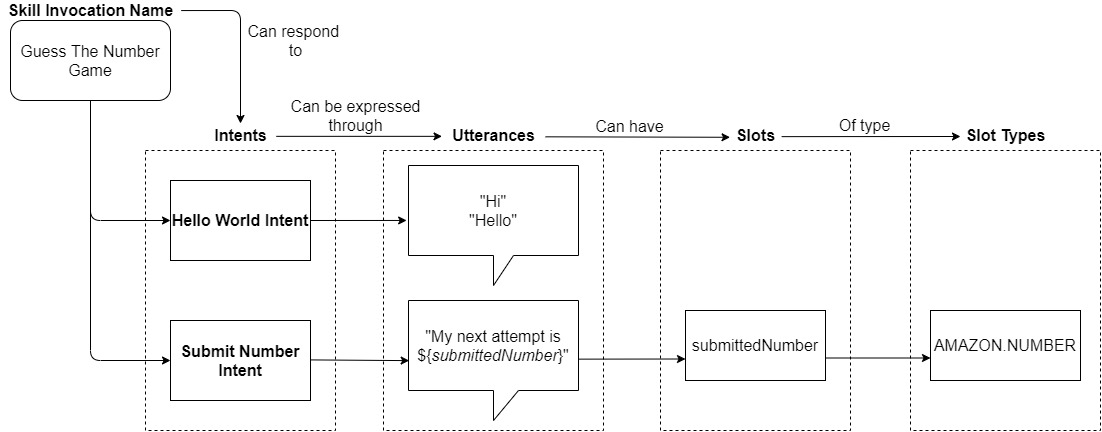
\includegraphics[scale=0.41]{resources/images/other/alexa-skill-dialog-model.jpg}
  \caption{Le componenti del modello di dialogo di una \textit{skill} di Alexa.}
  \label{fig:figure3.7}
\end{figure}
\hfill

\subsubsection{3.2.2.3. Il modello logico di una Alexa Skill}
\label{subsec:Sezione3.2.2.3}

Il modello logico di una \textit{skill} è costituito dal codice situato
nell’\textit{endpoint} della \textit{skill}. In generale, le richieste che il
cloud Alexa esegue sull’\textit{endpoint} sono semplici richieste \textit{http
post}, che possono essere gestite liberamente. Tuttavia, Amazon predispone e
suggerisce l’uso del suo framework, chiamato \textbf{ASK SDK} \cite{ASK_SDK},
che predilige una logica ad \textit{handler di eventi}, o, nello specifico, ad
\textit{handler d'intenzioni} (\textit{\textbf{intent handlers}}). In aggiunta,
il framework offre diverse funzionalità, tra cui la \textit{validazione delle
richieste}, ovvero una verifica sul mittente delle richieste ricevute
dall’\textit{endpoint}, che garantisca la loro provenienza dal cloud di Alexa
(requisito necessario al deployment della \textit{skill}).

\subsection{Comunicazione tra Alexa e OpenHAB}
\label{subsec:Sezione3.2.3}

In questo capitolo, si descriverà come è stata realizzata la comunicazione
bidirezionale tra Alexa e OpenHAB, attraverso i servizi che offrono per
interfacciarsi l’uno con l’altro.

\subsubsection{3.2.3.1. Amazon Echo Control Binding per OpenHAB}
\label{subsec:Sezione3.2.3.1}

\textbf{Amazon Echo Control Binding} \cite{BINDING_AECB} è un \textit{add-on}
di OpenHAB che permette d'integrare un dispositivo Alexa al sistema OpenHAB.
Il \textit{binding} sarà quindi utilizzato per gestire la comunicazione
\textbf{da OpenHAB verso Alexa}.

Più in dettaglio, consente di collegare degli account Amazon a OpenHAB e
pertanto di controllare i dispositivi Alexa associati a quegli account, come se
fossero delle \textit{things}. Risulta dunque possibile utilizzare un
\textit{Alexa Echo Dot} per dare voce al proprio sistema domotico, inviando
notifiche vocali di eventi rilevati da OpenHAB.

\subsubsection{3.2.3.2. OpenHAB Skill per Alexa}
\label{subsec:Sezione3.2.3.2}

\textbf{OpenHAB} \cite{OPENHAB_SKILL} è anche il nome di una \textit{skill} per
Alexa, che permette di mappare ogni dispositivo connesso a OpenHAB alle
interfacce predisposte da Alexa, che descrivono le capacità di un certo
dispositivo, consentendo così un’interazione vocale verso di esso. La
\textit{skill} sarà perciò utilizzata per gestire la comunicazione
\textbf{da Alexa verso OpenHAB}.

\section{Limitazioni del progetto}
\label{sec:Sezione3.3}

Ora si illustreranno alcune delle limitazioni del sistema, dovute stavolta alla
particolare progettazione scelta.

La prima limitazione è dovuta ai protocolli di comunicazione utilizzati.
Infatti, gran parte delle comunicazioni nel sistema avvengono tramite il
protocollo \textit{http}, che è un protocollo particolarmente lento e pesante
su dispositivi con poche risorse per la computazione. Questo provocherà una
certa \textbf{latenza nelle interazioni con il proprio sistema domotico}, in
particolare le interazioni vocali, che sono le più complesse.

La seconda limitazione è dovuta alla \textbf{non scalabilità del servizio
pubblico per gli esercizi cognitivi}, che è installato su un singolo server.
Trattandosi di un servizio pubblico, la cui domanda potrebbe variare molto nel
tempo, la sua scalabilità risulta un fattore necessario. Nonostante ciò, il
singolo server si presta bene almeno allo studio e alla realizzazione di un
prototipo.

La terza limitazione è dovuta al metodo con cui è stato esposto il server
locale, per offrire un servizio pubblico. Infatti, utilizzare il servizio
\textit{ngrok} aggiunge un ulteriore intermediario nella comunicazione,
aumentando dunque la latenza nelle interazioni con il proprio servizio. Inoltre
la licenza gratuita di \textit{ngrok} non concede di dare un nome pubblico al
proprio server, ma restituisce un identificatore casuale.